\documentclass[12pt]{article}

\usepackage[T1]{fontenc}
\usepackage{amsthm} % before newtxmath b/c latex
\usepackage{amsmath}
\usepackage{amsfonts}
\usepackage[scr]{rsfso}
\usepackage{bm}
\usepackage{thmtools}
\usepackage{mathtools}
\usepackage{enumitem}
\usepackage{hyperref}
\usepackage{cancel}
\usepackage{empheq}
\usepackage{listings}
\usepackage{booktabs}

\usepackage{tikzit}
\input{pm.tikzstyles}

\usepackage[parfill]{parskip}
\setlength{\parindent}{0pt}
\setlength{\parskip}{2ex plus 0.2ex minus 0.2ex}

\usepackage[
paper  = letterpaper,
left   = 1in,
right  = 1in,
top    = 1in,
bottom = 1in,
]{geometry}

\definecolor{codegreen}{rgb}{0,0.6,0}
\definecolor{codegray}{rgb}{0.5,0.5,0.5}
\definecolor{codepurple}{rgb}{0.58,0,0.82}

\lstdefinestyle{mystyle}{
    commentstyle=\color{codegreen},
    keywordstyle=\color{magenta},
    numberstyle=\tiny\color{codegray},
    stringstyle=\color{codepurple},
    basicstyle=\ttfamily\footnotesize,
    breakatwhitespace=false,         
    breaklines=true,                 
    captionpos=b,                    
    keepspaces=true,                 
    numbers=left,                    
    numbersep=5pt,                  
    showspaces=false,                
    showstringspaces=false,
    showtabs=false,                  
    tabsize=2
}

\lstset{
    style=mystyle
}


\newcommand{\N}{\mathbb{N}}
\newcommand{\Z}{\mathbb{Z}}
\newcommand{\Q}{\mathbb{Q}}
\newcommand{\R}{\mathbb{R}}
\newcommand{\C}{\mathbb{C}}

\newcommand{\iid}{\overset{iid}{\sim}}

\title{
    STCS 6701: Probabilistic Machine Learning \\
    Homework 1%
}
\author{
    Satvik Saha ({\tt ss7228})%
}
\date{
    \vspace{-1.2em}
    \today%
}

\begin{document}

\maketitle


% \tableofcontents

\section*{Question 1}

Fix $N, K \in \N$, $m_0, \tau_0^2 \in \R$, $\{\sigma_k^2\}_{k = 1}^K \subset
\R$, and consider finite Gaussian mixture model
\begin{align*}
    \mu_k &\sim \text{Normal}(m_0, \tau_0^2), & 1 \leq k \leq K, \\
    z_i &\sim \text{Categorical}(\bm{1}/K), & 1 \leq i \leq N, \\
    x_i \mid z_i = k, \mu_k &\sim \text{Normal}(\mu_k, \sigma_k^2), & 1 \leq i \leq N.
\end{align*}
This gives the joint density \begin{align*}
    p(\bm{x}, \bm{z}, \bm{\mu})
        &= \prod_k p(\mu_k) \cdot \prod_i p(z_i)\, p(x_i \mid z_i, \bm{\mu}) \\
        &\propto \prod_k \phi(\mu_k; m_0, \tau_0^2) \cdot \prod_{i, k} \phi(x_i; \mu_k, \sigma_k^2)^{z_{ik}} \\
        &\propto \prod_k (2\pi\sigma_k^2)^{-N_k /2} \exp\left(-\frac{1}{2\tau_0^2}(\mu_k - m_0)^2 - \frac{1}{2\sigma_k^2} \sum_{i} z_{ik}(x_i - \mu_k)^2\right), \tag{$\star$} \label{Q1_joint}
\end{align*}
with the shorthand $z_{ik} := \bm{1}(z_i = k)$, and \[
    \phi(t; \mu, \sigma^2) := \frac{1}{\sqrt{2\pi\sigma^2}}\, e^{-(t - \mu)^2 / 2\sigma^2}.
\] Note that $p(z_i) = \prod_k (1 /K)^{z_{ik}} = 1 /K$ is a constant.

% For each $k$, further set \begin{align*}
%     I_k &= \{i: z_i = k\}, &
%     N_k &= |I_k| = \sum_i z_{ik}, \\
%     S_k^{(1)} &= \sum_{i \in I_k} x_i = \sum_i x_i z_{ik}, &
%     \bar{x}_k &= \frac{S_k^{(1)}}{N_k}.
% \end{align*}

\subsection*{Part A}
\begin{enumerate}[label=(\alph*)]
    \item Fixing all quantities apart from $z_i$ in the joint \eqref{Q1_joint} gives
    the complete conditional \[
        p(z_i\mid -)
            \propto \prod_k (2\pi\sigma_k^2)^{-z_{ik}/2}\exp\left(-\frac{1}{2\sigma_k^2} z_{ik}(x_i - \mu_k)^2\right),
    \] which means that each \[
        p(z_i = k \mid -) \propto (2\pi\sigma_k^2)^{-1 /2}\exp\left(-\frac{(x_i - \mu_k)^2}{2\sigma_k^2}\right).
    \] Denoting $M_{ik}^2 := (x_i - \mu_k)^2 /\sigma_k^2$, we have \[
        \boxed{
            z_i \mid x_i, \bm{\mu}
                \sim \text{Categorical}\left(\left\{ \frac{\sigma_k^{-1} e^{-M_{ik}^2 / 2}}{\sum_{k'} \sigma_k^{-1} e^{-M_{ik'}^2 / 2}} \right\}_{k = 1}^K\right).
        }
    \]

    \item Fixing all quantities apart from $\mu_k$ in the joint \eqref{Q1_joint} gives
    the complete conditional \begin{align*}
        p(\mu_k \mid -)
            &\propto \exp\left(-\frac{1}{2\tau_0^2}(\mu_k - m_0)^2 - \frac{1}{2\sigma_k^2} \sum_{i} z_{ik}(x_i - \mu_k)^2\right) \\
            &= \exp\left(-\frac{1}{2\tau_0^2}(\mu_k - m_0)^2 - \frac{N_k}{2\sigma_k^2} (\mu_k - \bar{x}_k)^2 - \cancel{\frac{1}{2\sigma_k^2}\sum_{i \in I_k} (x_i - \bar{x}_k)^2}\right) \\
            &\propto \exp\left(-\frac{1}{2}\left(\frac{1}{\tau_0^2} + \frac{N_k}{\sigma_k^2}\right)\left(\mu_k - \frac{m_0 / \tau_0^2 + N_k \bar{x}_k / \sigma_k^2}{1/\tau_0^2 + N_k /\sigma_k^2}\right)^2\right).
    \end{align*}
    The second line uses $\sum_{i \in I_k} (x_i - \bar{x}_k)\mu_k = 0$.
    The third line involves `completing the square' in $\mu_k$.
    Thus, \[
        \boxed{\mu_k \mid \bm{x}, \bm{z} \sim \text{Normal}\left(\frac{m_0 / \tau_0^2 + S_k^{(1)} / \sigma_k^2}{1/\tau_0^2 + N_k /\sigma_k^2},\, \frac{1}{1/\tau_0^2 + N_k /\sigma_k^2}\right).}
    \]
\end{enumerate}

\subsection*{Part B}
\begin{enumerate}[label=(\alph*), resume]
    \item Conditioning on $\bm{z}$, our model is equivalent to $\mu_k \sim
    \text{Normal}(m_0, \tau_0^2)$, then sampling clusters $X_k \iid
    \text{Normal}(\mu_k, \sigma_k^2)$ independently of one another, where $X_k
    = \{x_i: z_i = k\}$: this can be seen by noting that the joint density of
    this model, proportional to \[
        \prod_k (2\pi\sigma_k^2)^{-N_k/2}\exp\left(-\frac{1}{2\tau^2}(\mu_k - m_0)^2 - \frac{1}{2\sigma_k^2}\sum_{i \in I_k} (x_i - \mu_k)^2\right),
    \] is identical to \eqref{Q1_joint} conditioned on $\bm{z}$.
    Thus, $p(\bm{x}, \bm{\mu} \mid \bm{z}) = \prod_k p(X_k, \mu_k \mid \bm{z})$
    factors across clusters, and (Fact 1) shows that integrating out
    $\mu_k$ from $p(X_k, \mu_k \mid \bm{z})$ gives \[
        \boxed{p(X_k \mid \bm{z})
            = (2\pi\sigma_k^2)^{-N_k /2} \left(\frac{\tau_0^2}{N_k\tau_0^2 + \sigma_k^2}\right)^{1 /2}
            \exp\left(-\frac{1}{2\sigma_k^2}\sum_{i \in I_k}(x_i - \bar{x}_k)^2 - \frac{N_k(\bar{x}_k - m_0)^2}{2(\sigma_k^2 + N_k \tau_0^2)}\right).}
    \] This also means that the collapsed marginal $p(\bm{x} \mid \bm{z}) =
    \prod_k p(X_k \mid \bm{z})$ factors across clusters.


    \item Since $p(\bm{z}) = \prod_{ik}(1 /K)^{z_{ik}} = 1 /K^N$ is a constant,
    we have \[
        p(\bm{x}, \bm{z})
            = p(\bm{x} \mid \bm{z})\, p(\bm{z})
            \propto \prod_k p(X_k\mid \bm{z}),
    \] so \[
        p(z_i = k\mid \bm{x}, \bm{z}_{-i})
            \propto \prod_k p(X_k\mid \bm{z}_{-i}, z_i = k) =: p_{ik},
    \] where the right hand side is evaluated as in the previous part, forcing
    $x_i$ into the $k$-th component.
    This means that for terms $p(X_{k'}\mid z_{-i}, z_i = k)$ with $k' \neq k$,
    the quantities $N_{k'}, \bar{x}_{k'}$ in the boxed equation in the previous
    part are really $N_{k', -i}, \bar{x}_{k', -i}$ with the sum taken over
    $I_{k'}\setminus\{i\}$; if $N_{k', -i} = 0$, the expression remains valid.
    Similarly, if $N_{k, -i} = 0$, the $k$-th term uses $N_k = 1$, $\bar{x}_{k}
    = x_i$, and the expression remains valid (reducing to the normal prior
    predictive density proportional to $p(x_i\mid z_i, \mu_k)\, p(\mu_k)$).

    Normalizing, we have \[
        \boxed{
            p(z_i = k \mid \bm{x}, \bm{z}_{-i})
                = \frac{p_{ik}}{\sum_{k'} p_{ik'}}.
        }
    \]
    % This means that the posterior predictive density under component $k$ is
    % described by
    % \begin{align*}
    %     p_{\text{pred}}(x_i \mid X_{k, -i})
    %         &\propto (2\pi\sigma_k^2)^{-N_{k, -i} /2} \left(\frac{\tau_0^2}{N_{k, -i}\tau_0^2 + \sigma_k^2}\right)^{1 /2} \\
    %         &\qquad\exp\left(-\frac{1}{2\sigma_k^2}\sum_{j \in I_k\setminus\{i\}}(x_j - \bar{x}_{k, -i})^2 - \frac{N_{k, -i}(\bar{x}_{k, -i} - m_0)^2}{2(\sigma_k^2 + N_{k, -i} \tau_0^2)}\right).
    % \end{align*}
\end{enumerate}


\subsection*{Part D}
\begin{enumerate}[label=(\alph*), resume]
    \item The given model can be drawn using plate notation as follows.
    \ctikzfig{simple_gmm}
\end{enumerate}




\clearpage
\section*{Question 2}

Fix $N, K \in \N$, $m_0 \in \R$, $a_0, b_0, \kappa_0 \in \R_+$,
$\{\alpha_k\}_{k = 1}^K \subset \R_+$ and consider the model
\begin{align*}
    \pi &\sim \text{Dirichlet}(\alpha_1, \dots, \alpha_K), \\
    \lambda_k &\sim \text{Gamma}(a_0, b_0), & 1 \leq k \leq K, \\
    \mu_k \mid \lambda_k &\sim \text{Normal}(m_0, (\kappa_0\lambda_k)^{-1}), & 1 \leq k \leq K, \\
    z_i \mid \pi &\sim \text{Categorical}(\pi_1, \dots, \pi_K), & 1 \leq i \leq N, \\
    x_i \mid z_i = k, \mu_k, \lambda_k &\sim \text{Normal}(\mu_k, \lambda_k^{-1}), & 1 \leq i \leq N.
\end{align*}
This gives the joint density \begin{align*}
    p(\bm{x}, \bm{z}, \bm{\mu}, \bm{\lambda}, \pi)
        &= p(\pi) \prod_k p(\lambda_k)\, p(\mu_k\mid \lambda_k)\prod_i p(z_i \mid \pi)\, p(x_i \mid z_i, \bm{\mu}, \bm{\lambda}) \\
        &\propto \prod_k \pi_k^{\alpha_k - 1} \cdot \prod_k \lambda_k^{a_0 - 1} e^{-b_0\lambda_k} \cdot \lambda_k^{1 /2} e^{-\kappa_0\lambda_k(\mu_k - m_0)^2 /2} \\
            &\qquad \cdot \prod_{ik} \pi_k^{z_{ik}} \lambda_k^{z_{ik} /2} e^{-z_{ik}\lambda_k (x_i - \mu_k)^2 / 2} \\
        &\propto \prod_k \pi_k^{\alpha_k + N_k - 1} \cdot \prod_k \lambda_k^{a_0 + N_k / 2 - 1 /2} \\
            &\qquad \cdot \prod_k \exp\left(-b_0\lambda_k -\frac{1}{2}\kappa_0\lambda_k(\mu_k - m_0)^2 -\frac{1}{2}\lambda_k\sum_i z_{ik}(x_i - \mu_k)^2\right)
            \tag{$\star\star$} \label{Q2_joint}
\end{align*}

\subsection*{Part A}
\begin{enumerate}[label=(\alph*)]
    \item Fixing all quantities apart from $\pi$ in the joint \eqref{Q2_joint}
    gives the complete conditional \[
        p(\pi\mid - ) \propto \prod_k \pi_k^{\alpha_k + N_k - 1},
    \] which we identify as a Dirichlet density with parameters $\{\alpha_k +
    N_k\}_{k = 1}^K$, so \[
        \boxed{
            \pi \mid \bm{z} \sim \text{Dirichlet}(\alpha_1 + N_1, \dots, \alpha_k + N_k),
        }
    \] with density \[
        \boxed{
            p(\pi\mid \bm{z}) = \frac{\prod_k \Gamma(\alpha_k + N_k)}{\Gamma(\sum_k \alpha_k + N)} \prod_k \pi_k^{\alpha_k + N_k - 1}.
        }
    \]

    \item Fixing all quantities apart from $\mu_k$ in the joint
    \eqref{Q2_joint} gives \begin{align*}
        p(\mu_k \mid -)
            &\propto \exp\left(-\frac{1}{2}\kappa_0\lambda_k(\mu_k - m_0)^2 -\frac{1}{2}\lambda_k\sum_i z_{ik}(x_i - \mu_k)^2\right) \\
            &\propto \exp\left(-\frac{1}{2}\kappa_0\lambda_k(\mu_k - m_0)^2 -\frac{1}{2}\lambda_k N_k (\mu_k - \bar{x}_k)^2 - \cancel{\frac{1}{2}\lambda_k\sum_{i \in I_k} (x_i - \bar{x}_k)^2}\right) \\
            &\propto \exp\left(-\frac{1}{2}\lambda_k\left(\kappa_0 + N_k\right)\left(\mu_k - \frac{\kappa_0 m_0 + N_k\bar{x_k}}{\kappa_0 + N_k}\right)^2\right).
    \end{align*}
    Thus, \[
        \boxed{
            \mu_k \mid \lambda_k, \bm{x}, \bm{z} \sim \text{Normal}\left(\frac{\kappa_0m_0 + N_k\bar{x}_k}{\kappa_0 + N_k},\, \frac{1}{\lambda_k(\kappa_0 + N_k)}\right).
        }
    \]

    \item Fixing all quantities apart from $\lambda_k$ in the joint
    \eqref{Q2_joint} gives \begin{align*}
        p(\lambda_k \mid -)
            &\propto \lambda_k^{a_0 + N_k / 2 - 1 /2}
                \exp\left(-b_0\lambda_k -\frac{1}{2}\kappa_0\lambda_k(\mu_k - m_0)^2 -\frac{1}{2}\lambda_k\sum_i z_{ik}(x_i - \mu_k)^2\right),
    \end{align*}
    which we identify as a Gamma density, whose rate parameter simplifies as
    \begin{align*}
        &b_0 + \frac{1}{2}\kappa_0(\mu_k - m_0)^2 + \frac{1}{2}\sum_{i \in I_k}\left(x_i^2 - 2\mu_k x_i + \mu_k^2\right) \\
            = \;&b_0 + \frac{1}{2}\kappa_0(\mu_k - m_0)^2 + \frac{1}{2}S_k^{(2)} - \mu_k S_k^{(1)} + \frac{1}{2}N_k\mu_k^2.
    \end{align*}
    Thus, \[
        \boxed{
            \lambda_k \mid \mu_k, \bm{x}, \bm{z} \sim \text{Gamma}\left(
                a_0 + \frac{1}{2}N_k + \frac{1}{2},\,
                b_0 + \frac{1}{2}\kappa_0(\mu_k - m_0)^2 + \frac{1}{2}S_k^{(2)} - \mu_k S_k^{(1)} + \frac{1}{2}N_k\mu_k^2
            \right).
        }
    \]

    \item Fixing all quantities apart from $z_i$ in the joint \eqref{Q2_joint}
    gives \[
        p(z_i \mid -)
            \propto \prod_k \pi_k^{z_{ik}} \lambda_k^{z_{ik}/2} \exp\left(-\frac{1}{2}\lambda_k z_{ik}(x_i - \mu_k)^2\right),
    \] which means that \[
        p(z_i = k \mid -)
            \propto \pi_k\lambda_k^{1/2} \exp\left(-\frac{1}{2}\lambda_k (x_i - \mu_k)^2\right).
    \] Denoting $M_{ik}^2 := \lambda_k (x_i - \mu_k)^2$, we have \[
        \boxed{
            z_i \mid x_i, \bm{\mu}, \bm{\lambda}, \pi
                \sim \text{Categorical}\left(\left\{ \frac{\pi_k \lambda_k^{1 /2} e^{-M_{ik}^2 / 2}}{\sum_{k'}\pi_{k'} \lambda_{k'}^{1 /2} e^{-M_{ik'}^2 / 2}} \right\}_{k = 1}^K\right).
        }
    \] 
\end{enumerate}

\subsection*{Part B}
\begin{enumerate}[label=(\alph*), resume]
    \item Write \begin{align*}
        p(\mu_k, \lambda_k &\mid D_{k, -i}) \\
            &\propto p(\lambda_k)\, p(\mu_k\mid \lambda_k)\, p(D_{k, -i} \mid \mu_k, \lambda_k) \\
            &\propto \lambda_k^{a_0 - 1} e^{-b_0\lambda_k}\cdot \lambda_k^{1 /2} e^{-\kappa_0\lambda_k(\mu_k - m_0)^2 /2}
                \cdot \prod_{j \in I_k\setminus\{i\}} \lambda_k^{1 /2} e^{-\lambda_k(x_j - \mu_k)^2 /2} \\
            &\propto \lambda_k^{a_0 + N_{k, -i}/2 - 1 /2}
                \cdot \exp\left(-b_0\lambda_k -\frac{1}{2}\kappa_0\lambda_k(\mu_k - m_0)^2 -\frac{1}{2}\lambda_k\sum_{j \in I_k\setminus\{i\}}(x_j - \mu_k)^2\right) \\
            &\propto \lambda_k^{a_0 + N_{k, -i}/2 - 1 /2}
                \cdot \exp\Bigg(-b_0\lambda_k -\frac{1}{2}\kappa_0\lambda_k(\mu_k - m_0)^2 \\
                &\qquad -\frac{1}{2}\lambda_kN_{k, -i}(\mu_k - \bar{x}_{k, -i})^2  -\frac{1}{2}\lambda_k\sum_{j \in I_k\setminus\{i\}}(x_j - \bar{x}_{k, -i})^2\Bigg) \\
            &\propto \lambda_k^{a_0 + N_{k, -i}/2 - 1 /2}
                \cdot \exp\Bigg(-b_0\lambda_k -\frac{1}{2}\lambda_k(\kappa_0 + N_{k, -i})\left(\mu_k - \frac{\kappa_0m_0 + N_{k, -i}\bar{x}_{k, -i}}{\kappa_0 + N_{k, -i}}\right)^2 \\
                    &\qquad +\frac{1}{2}\lambda_k \frac{(\kappa_0m_0 + N_{k, -i}\bar{x}_{k, -i})^2}{\kappa_0 + N_{k, -i}}
                        -\frac{1}{2}\lambda_k\kappa_0 m_0^2 -\frac{1}{2}\lambda_kN_{k, -i}\bar{x}_{k, -i}^2 \\
                    &\qquad -\frac{1}{2}\lambda_k\sum_{j \in I_k\setminus\{i\}}(x_j - \bar{x}_{k, -i})^2\Bigg) \\
            &\propto \lambda_k^{a_0 + N_{k, -i}/2 - 1 /2}
                \cdot \exp\Bigg(-b_0\lambda_k -\frac{1}{2}\lambda_k(\kappa_0 + N_{k, -i})\left(\mu_k - \frac{\kappa_0m_0 + N_{k, -i}\bar{x}_{k, -i}}{\kappa_0 + N_{k, -i}}\right)^2 \\
                    &\qquad -\frac{1}{2}\lambda_k \frac{\kappa_0N_{k, -i}(m_0 - \bar{x}_{k, -i})^2}{\kappa_0 + N_{k, -i}}
                    -\frac{1}{2}\lambda_k\sum_{j \in I_k\setminus\{i\}}(x_j - \bar{x}_{k, -i})^2\Bigg) \\
            &\propto \lambda_k^{a_0 + N_{k, -i}/2 - 1}
                \exp\left(-b_0\lambda_k -\frac{1}{2}\lambda_k \frac{\kappa_0N_{k, -i}(m_0 - \bar{x}_{k, -i})^2}{\kappa_0 + N_{k, -i}} -\frac{1}{2}\lambda_k\sum_{j \in I_k\setminus\{i\}}(x_j - \bar{x}_{k, -i})^2\right) \\
                &\quad\cdot \lambda_k^{1 /2}\exp\left(-\frac{1}{2}\lambda_k(\kappa_0 + N_{k, -i})\left(\mu_k - \frac{\kappa_0m_0 + N_{k, -i}\bar{x}_{k, -i}}{\kappa_0 + N_{k, -i}}\right)^2\right).
    \end{align*}
    \textit{%
        Using $p(\mu_k\mid\lambda_k)\,p(D_{k, -i}\mid \mu_k, \lambda_k) =
        p(D_{k, -i} \mid \lambda_k)\, p(\mu_k\mid D_{k, -i}, \lambda_k)$ with
        (Fact 1) would have saved a lot of algebra!
    }

    This factorizes precisely as \begin{align*}
            \lambda_k \mid D_{k, -i} &\sim \text{Gamma}(a_{k, -i}, b_{k, -i}), \\
            \mu_k \mid \lambda_k, D_{k, -i} &\sim \text{Normal}(m_{k, -i}, (\kappa_{k, -i}\lambda_{k})^{-1}),
    \end{align*}
    with the updated parameters \begin{empheq}[box=\fbox]{align*}
        a_{k, -i} &= a_0 + \frac{1}{2}N_{k, -i}, \\
        b_{k, -i} &= b_0 + \frac{1}{2}\frac{\kappa_0N_{k, -i}(m_0 - \bar{x}_{k, -i})^2}{\kappa_0 + N_{k, -i}} + \frac{1}{2} \sum_{j \in I_k\setminus\{i\}}(x_j - \bar{x}_{k, -i})^2 \\
        m_{k, -i} &= \frac{\kappa_0m_0 + N_{k, -i}\bar{x}_{k, -i}}{\kappa_0 + N_{k, -i}} \\
        \kappa_{k, -i} &= \kappa_0 + N_{k, -i}.
    \end{empheq}
    In the case $N_{k, -i} = 0$, conditioning on $D_{k, -i}$ is redundant, and
    $p(\mu_k, \lambda_k \mid D_{k, -i})$ is merely the prior distribution of
    $\mu_k, \lambda_k$.
    This gives precisely the same result as above, with the updates $(a_{k,
    -i}, b_{k, -i}, m_{k, -i}, \kappa_{k, -i}) = (a_0, b_0, m_0, \kappa_0)$
    corresponding exactly to plugging in $N_{k, -i} = 0$ and $I_k\setminus\{i\}
    = \emptyset$.

    Note that we may simplify \[
        \sum_{j \in I_k\setminus \{i\}} (x_j - \bar{x}_{k, -i})^2
            = S_{k, -1}^{(2)} - N_{k, -i} \bar{x}_{k, -i}^2.
    \]


    \item Using the above computation and (Fact 2), we immediately have the
    posterior predictive distribution under component $k$ described by \[
    \boxed{
        x_i\mid D_{k, -i} \sim t_{\nu_{k, -i}}(m_{k, -i}, s_{k, -i}^2), \qquad
        \nu_{k, -i} = 2a_{k, -i}, \quad
        s_{k, -i}^2 = \frac{b_{k, -i}}{a_{k, -i}} \cdot \frac{\kappa_{k, -i} + 1}{\kappa_{k, -i}}.
    }
    \]
    This remains true when $N_{k, -i} = 0$.
    The density can be explicitly written as \[
        p_{\text{pred}}(x_i\mid D_{k, -i})
            = \frac{\Gamma((\nu_{k, -i} + 1) / 2)}{\Gamma(\nu_{k, -i} / 2)\,\sqrt{\pi\nu_{k, -i}s_{k, -i}^2}}\,
                \left(1 + \frac{(x_i - m_{k, -i})^2}{\nu_{k, -i}s_{k, -i}^2}\right)^{-(\nu_{k, -i} + 1) / 2}.
    \]


    \item Write \[
        p(z_i = k \mid \bm{x}, \bm{z}_{-i}, \pi)
            \propto p(z_i = k\mid \pi)\, p_{\text{pred}}(x_i \mid D_{k, -i}),
    \] where $p_{\text{pred}}(x_i\mid D_{k, -i})$ is a $t$-density as described
    in the previous part.
    Normalizing, \[
    \boxed{
        p(z_i = k\mid \bm{x}, \bm{z}_{-i}, \pi)
            = \frac{\pi_k\, p_{\text{pred}}(x_i\mid D_{k, -i})}{\sum_{k'} \pi_{k'}\, p_{\text{pred}}(x_i\mid D_{k', -i})}
    }
    \]
\end{enumerate}


\subsection*{Part C}

This model is much more flexible than the one in Q1: the model allows for
different cluster proportions $\pi$, as well as learned cluster precisions
$\lambda_k$ (as opposed to assuming known precisions $\sigma_k^{-2}$).

In the blocked label update $z_i \mid x_i, \bm{\mu}, \bm{\lambda}, \pi$, the
cluster proportions $\pi$ bias $z_i\mid -$ towards larger clusters, relative to
purely using the normal likelihoods $\lambda_k^{1 /2}e^{-M_{ik}^2 /2}$ (like in
the label updates in Q1(a)).

The parameter $\lambda_k$ controls the cluster precision for component $k$;
lower values makes the mean update $\mu_k\mid -$ more variable, and flattens
out the terms $\pi_k\lambda_k^{1 /2}e^{-M_{ik}^2 /2}$ controlling the label
updates making them more uncertain as well.

The posterior predictive under a given component $k$ is now a $t$-distribution
(with degrees of freedom $2a_0 + N_{k, -i}$) instead of a normal, i.e.\ has
heavier tails (especially when the cluster size is small); this makes sense
since the (unknown) precision for the cluster mean $\mu_k$ is lower, the
cluster precision $\kappa_{k, -i}\lambda_k$ is also lower.


\subsection*{Part D}
\begin{enumerate}[label=(\alph*), resume]
    \item The given model can be drawn using plate notation as follows.
    \ctikzfig{gmm}
\end{enumerate}



\clearpage

\section*{Question 3}

We select the Gaussian mixture model from Question 2, with a Dirichlet prior on
mixture proportions $\pi$, Normal-Gamma priors on the component means and
precisions $\mu_k, \lambda_k$.
Using the work done there, we implement blocked and collapsed Gibbs samplers.
Using $\bm{\theta}$ to denote the collection of all latent variables
($(\bm{\lambda}, \bm{\mu}, \bm{z}, \pi)$ for the blocked sampler, only
$(\bm{z}, \pi)$ for the collapsed sampler), we thus obtain posterior sample
$\{\bm{\theta}_s\}$ over iterations $s$.

We generate synthetic data using the same generative process, with $N = 2000$,
$K = 3$, $m_0 = 0$, $a_0 = 2$, $b_0 = 1$, $\kappa_0 = 0.1$, $\alpha =
\bm{1}/K$.
The true cluster means $\bm{\mu}$ are $(-2.47, 0.20, 3.73)$, precisions
$\bm{\lambda}$ are $(5.31, 1.40, 0.93)$, and proportions $\pi$ are $(0.31,
0.52, 0.17)$; see Figure~\ref{fig:Q3_hist} for a better visualization.
Only $N_{in} = 1500$ data points are used for fitting the model; $N_{out} =
500$ samples are held for evaluation.

When fitting the mixture model, we first use $K = 3$, $m_0 = 0$, $a_0 = 1$,
$b_0 = 1$, $\kappa_0 = 0.1$, $\alpha = \bm{1}/K$; we further initialize $\pi =
\bm{1}/K$, $\bm{z}$ uniformly randomly on $\{1, \dots, K\}$ (for the both
samplers), and $\bm{\lambda} = \bm{1}$, $\bm{\mu} = \bm{0}$ (for the blocked
sampler).
The hyperparameters are chosen to be relatively non-informative; given that we
have a large amount of data, these choices are mostly immaterial and do not
affect the fit.

A summary of the training data $\bm{x}_{in}$ along with the fitted clusters
have been presented in Figure~\ref{fig:Q3_hist}.
We use $1000$ posterior samples, obtained after a burn-in period of $1000$
iterations.
A trace plot of the cluster centers as in Figure~\ref{fig:Q3_log_joint} (right)
shows that \emph{label switching} does not occur in this run, hence we simply
use the mode of the samples of $z_i \mid \bm{x}_{in}$ as the fitted cluster
label for $x_i$.

We further re-run $8$ chains for each sampler, and monitor the log joint
density $\log{p(\bm{x}_{in}, \bm{\theta}_s)}$ over iterations $s$; this has
been presented in Figure~\ref{fig:Q3_log_joint} (left).
Since all chains eventually hover around the same value, we are relatively
confident that our samplers have reached stationarity, well before the burn-in
period of $1000$ iterations.
The collapsed sampler seems to reach stationarity a little sooner than the
blocked sampler, but the effect is too small to report.


\begin{figure}
\begin{center}
    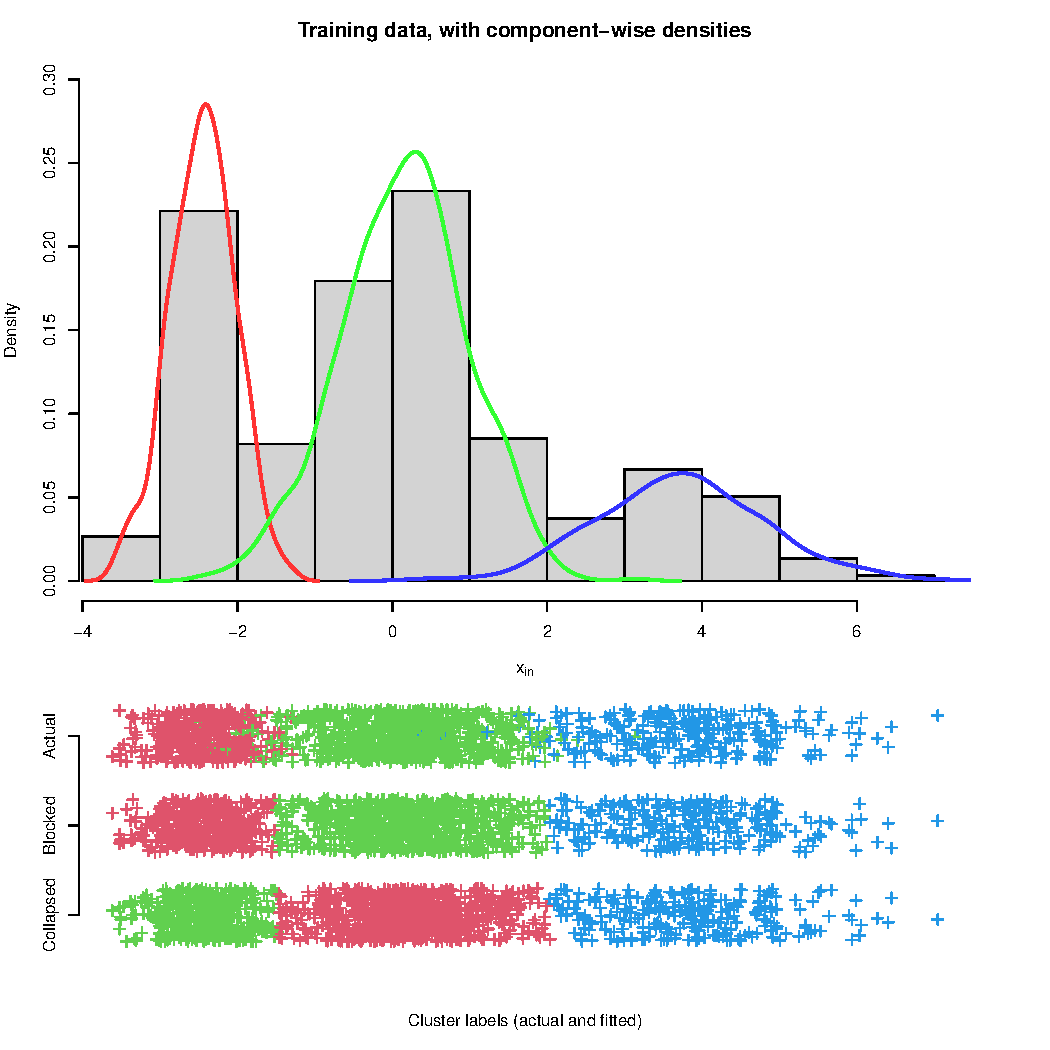
\includegraphics{gmm_Q3_hist_3}
\end{center}
\caption{
    \emph{Top}: Distribution of data $\bm{x}_{in}$ used to fit the model, with density
    plots of $\bm{x}_{in}$ for each of the $K = 3$ constituent components.
    \emph{Bottom}: Actual and fitted cluster labels (modes of $z_i\mid
    \bm{x}_{in}$ from posterior samples) in color.
    The points $\bm{x}_{in}$ have been vertically jittered.
    Note that both samplers recover the original clusters up to permutations.
}
\label{fig:Q3_hist}
\end{figure}



\begin{figure}
\begin{center}
    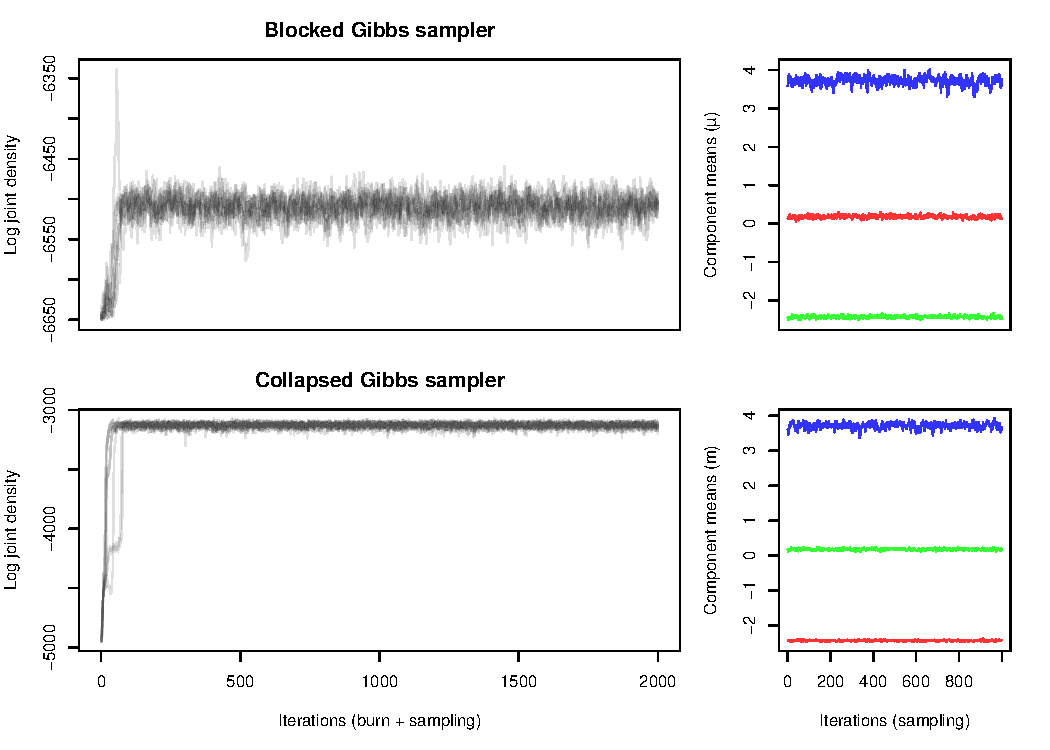
\includegraphics{gmm_Q3_logjoint_3}
\end{center}
\caption{
    \emph{Left}: Evolution of the log joint density $\log{p(\bm{x}_{in},
    \bm{\theta}_s)}$ over posterior samples $\{\bm{\theta}_s\}$ (including
    burn-in), for $8$ chains.
    \emph{Right}: Evolution of the cluster centers over sampling iterations for
    the first chain.
}
\label{fig:Q3_log_joint}
\end{figure}



One way of evaluating a fit is by estimating an \emph{Expected Log Predictive
Density} (ELPD) score \[
    \text{ELPD} := \mathbb{E}_{X \sim f}\left[\log{p(X \mid \bm{x}_{in})}\right],
\] where $f$ is the data generating distribution and the predictive density is
\[
    p(x\mid \bm{x}_{in})
        = \mathbb{E}_{\bm\theta \mid \bm{x}_{in}}\left[p(x\mid \bm{\theta})\right]
        = \int p(x\mid\bm{\theta})\, p(\bm{\theta} \mid \bm{x}_{in}) \:d\bm{\theta},
\]
Here, we estimate $p(x\mid \bm{x}_{in})$ by averaging the data likelihood
$p(x\mid \bm{\theta}_s)$ over posterior samples $\{\bm{\theta}_s\}$.
We further estimate the ELPD by averaging (the estimate of) $\log{p(x_o\mid
\bm{x}_{in})}$ over held out samples $\{x_o\}$ from $\bm{x}_{out}$, the latter
being a proxy for the data generating distribution $f$.
In the blocked Gibbs sampler, $p(x\mid \bm{\lambda}, \bm{\mu}, \pi)$ is a
$\pi$-mixture of $(\mu_k, \lambda_k^{-1})$-Gaussians ($\bm{z}$ is integrated
out), while in the collapsed Gibbs sampler, $p(x\mid \pi)$ is a $\pi$-mixture
of $t$-distributions (which are practically indistinguishable from Gaussians in
large components).

Estimates of ELPD have been presented in Figure~\ref{fig:Q3_elpd}.
We cannot detect any significant difference between the two samplers here.

\begin{figure}
\begin{center}
    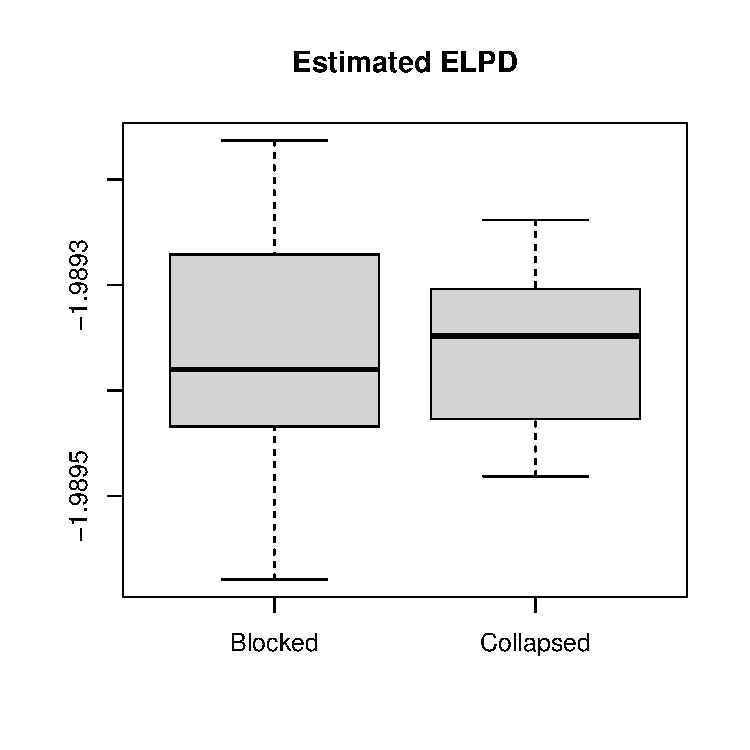
\includegraphics{gmm_Q3_elpd_3}
\end{center}
\caption{
    Estimates of ELPD for both samplers across 8 chains.
}
\label{fig:Q3_elpd}
\end{figure}












\clearpage
\begin{center}
{\LARGE
    Image segmentation with Gaussian mixtures:

    B\"ocklin's \emph{Isle of the Dead}
}
\end{center}
\vspace{2em}

\begin{abstract}
    We model the pixel intensity distribution of an image (Arnold B\"ocklin's
    \emph{Isle of the Dead}) with a finite Gaussian mixture.
    After fitting this model with $K = 4$ components using a collapsed Gibbs
    sampler, we reconstruct the image by replacing each pixel intensity with
    its cluster mean.
    The different cluster components are loosely interpreted as different
    segments of the image.
\end{abstract}
\vspace{1em}


\subsection*{Introduction}

Image segmentation generally describes the process of separating an image into
different groups or regions of pixels.
Pixels in a group share some similarities; for instance, they may belong to the
same `object' in the image scene.
A crude method of identifying separate objects in an image is to pick $K$
colors, then declare a pixel to be part of the $k$-th object if its color is
most similar to the $k$-th color.
In the case of a grayscale image with $N$ pixels, each pixel merely has a
one-dimensional intensity $x_i \in [0, 1]$: this method amounts to clustering
the image pixel intensities $\bm{x} = \{x_i\}_{i = 1}^N$ into $K$ components.

\begin{figure}[ht!]
\begin{center}
    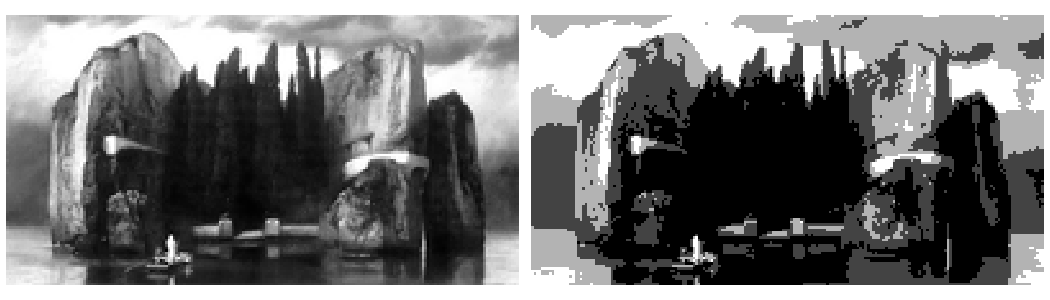
\includegraphics[width=\textwidth]{iotd}
\end{center}

\caption{
    \emph{Left}: Arnold B\"ocklin's \emph{Isle of the Dead}, fourth version,
    1884.
    This is a black-and-white photograph that has been converted to grayscale
    and scaled down to $200\times 105$ pixels. \\
    \emph{Right}: Segmented image --- pixel intensities are fitted as a mixture
    of $K = 4$ Gaussians, following which each pixel intensity is replaced by
    its cluster mean.
}
\label{fig:iotd}
\end{figure}

Here, we attempt to segment a grayscale image in this manner, using a finite
Gaussian mixture to model its intensity distribution.
The image we choose is Arnold B\"ocklin's painting \emph{Isle of the Dead}
(Figure~\ref{fig:iotd}, left), which has inspired numerous works of art, drama,
literature, and music.
This is a black-and-white photograph of his fourth version from 1884, which the
composer Sergei Rachmaninoff used as a basis for his symphonic poem \emph{Isle
of the Dead, Op.\ 29}.
Amusingly, when Rachmaninoff later saw the original (in color), he remarked
with disappointment that he would not have written his piece had he seen this
version first!
The resulting segmented image has been presented in Figure~\ref{fig:iotd}
(right).


It is important to note that this procedure only operates on the intensity
distribution of an image, and uses no information about where each pixel is
spatially situated in the image!
Thus, actual objects in an image can be distinguished only if they
significantly differ in color.
What we obtain here instead are regions of an image with each associated with a
certain brightness level; this is greatly affected by the presence of shadows
and highlights.



\subsection*{Model}

Fix $N, K \in \N$, $m_0 \in \R$, $a_0, b_0, \kappa_0 \in \R_+$,
$\{\alpha_k\}_{k = 1}^K \subset \R_+$ and consider the following generative
model for pixel intensities $\{x_i\}_{i = 1}^N$ in an image with $N$ pixels.
\begin{align*}
    \pi &\sim \text{Dirichlet}(\alpha_1, \dots, \alpha_K), \\
    \lambda_k &\sim \text{Gamma}(a_0, b_0), & 1 \leq k \leq K, \\
    \mu_k \mid \lambda_k &\sim \text{Normal}(m_0, (\kappa_0\lambda_k)^{-1}), & 1 \leq k \leq K, \\
    z_i \mid \pi &\sim \text{Categorical}(\pi_1, \dots, \pi_K), & 1 \leq i \leq N, \\
    x_i \mid z_i = k, \mu_k, \lambda_k &\sim \text{Normal}(\mu_k, \lambda_k^{-1}), & 1 \leq i \leq N.
\end{align*}
Here, $\text{Gamma}(\alpha, \beta)$ is shape-rate parametrized, and
$\text{Normal}(\mu, \sigma^2)$ is mean-variance parametrized.
This gives the joint density \begin{align*}
    p(\bm{x}, \bm{z}, \bm{\mu}, \bm{\lambda}, \pi)
        &= p(\pi) \prod_k p(\lambda_k)\, p(\mu_k\mid \lambda_k)\prod_i p(z_i \mid \pi)\, p(x_i \mid z_i, \bm{\mu}, \bm{\lambda}) \\
        % &\propto \prod_k \pi_k^{\alpha_k - 1} \cdot \prod_k \lambda_k^{a_0 - 1} e^{-b_0\lambda_k} \cdot \lambda_k^{1 /2} e^{-\kappa_0\lambda_k(\mu_k - m_0)^2 /2} \\
        %     &\qquad \cdot \prod_{ik} \pi_k^{z_{ik}} \lambda_k^{z_{ik} /2} e^{-z_{ik}\lambda_k (x_i - \mu_k)^2 / 2} \\
        &\propto \prod_k \pi_k^{\alpha_k + N_k - 1} \cdot \prod_k \lambda_k^{a_0 + N_k / 2 - 1 /2} \\
            &\qquad \cdot \prod_k \exp\left(-b_0\lambda_k -\frac{1}{2}\kappa_0\lambda_k(\mu_k - m_0)^2 -\frac{1}{2}\lambda_k\sum_{i \in I_k}(x_i - \mu_k)^2\right),
\end{align*}
where $I_k = \{i : z_i = k\}$, $N_k = |I_k|$ are functions of $\bm{z}$.
This can be described using plate notation as in Figure~\ref{fig:iotd_gmm}.

\begin{figure}[ht!]
    \ctikzfig{gmm}
\caption{The finite Gaussian mixture model under consideration, in plate notation}
\label{fig:iotd_gmm}
\end{figure}


\subsection*{Inference}

We use a blocked Gibbs sampler to obtain $S$ posterior samples from $\bm{z},
\pi \mid \bm{x}$.
This involves alternately sampling cluster proportions \[
    \pi\mid \bm{z}, \bm{x} \sim \text{Dirichlet}(\alpha_1 + N_1, \dots, \alpha_K + N_K),
\] and cluster labels \[
    p(z_i = k \mid \bm{z}_{-i}, \pi, \bm{x}) = \frac{\pi_k \, p_{\text{pred}}(x_i \mid D_{k, -i})}{\sum_{k'}\pi_{k'} \, p_{\text{pred}}(x_i \mid D_{k', -i})}.
\] Here, $p_{\text{pred}}(x_i\mid D_{k, -i})$ is the posterior predictive
density for component $k$ excluding the data point $x_i$, described by \[
    x_i\mid D_{k, -i} \sim t_{\nu_{k, -i}}(m_{k, -i}, s_{k, -i}^2), \qquad
        \nu_{k, -i} = 2a_{k, -i}, \quad
        s_{k, -i}^2 = \frac{b_{k, -i}}{a_{k, -i}} \cdot \frac{\kappa_{k, -i} + 1}{\kappa_{k, -i}},
\] with the updates \begin{align*}
    a_{k, -i} &= a_0 + \frac{1}{2}N_{k, -i}, \\
    b_{k, -i} &= b_0 + \frac{1}{2}\frac{\kappa_0N_{k, -i}(m_0 - \bar{x}_{k, -i})^2}{\kappa_0 + N_{k, -i}} + \frac{1}{2} \sum_{j \in I_k\setminus\{i\}}(x_j - \bar{x}_{k, -i})^2 \\
    m_{k, -i} &= \frac{\kappa_0m_0 + N_{k, -i}\bar{x}_{k, -i}}{\kappa_0 + N_{k, -i}} \\
    \kappa_{k, -i} &= \kappa_0 + N_{k, -i}.
\end{align*}
Here, $N_{k, -i} = |I_k\setminus\{i\}|$, and $\bar{x}_{k, -i} = \frac{1}{N_{k,
-i}}\sum_{j \in I_{k} \setminus\{i\}} x_j$ (set to $0$ if $N_{k, -i} = 0$).

Note that for a new data point, the likelihood $p(x_{N+1}\mid \bm{z}, \pi,
\bm{x})$ for a new data point $x_{N + 1}$ is a $\pi$-mixture of
$t$-distributions, each with the same parameters as described before.
The posterior predictive density $p(x_{N + 1} \mid \bm{x}) =
\mathbb{E}_{\bm{z}, \pi \mid \bm{x}}[p(x_{N + 1} \mid \bm{z}, \pi, \bm{x})]$ is
estimated by a Monte-Carlo average over posterior samples of $\bm{z}, \pi \mid
\bm{x}$.

The \emph{Expected Log Predictive Density} (ELPD) score \[
    \text{ELPD} := \mathbb{E}_{X \sim f}\left[\log{p(X \mid \bm{x}_{in})}\right],
\] where $f$ is the data generating distribution for $\bm{x}$, is estimated by
a Monte-Carlo average of $\log{p(x_o\mid \bm{x}_{in})}$ over held out samples
$\{x_o\}$ from our data $\bm{x}$; the latter is a proxy for the data generating
distribution $f$.



\begin{figure}[h!]
\begin{center}
    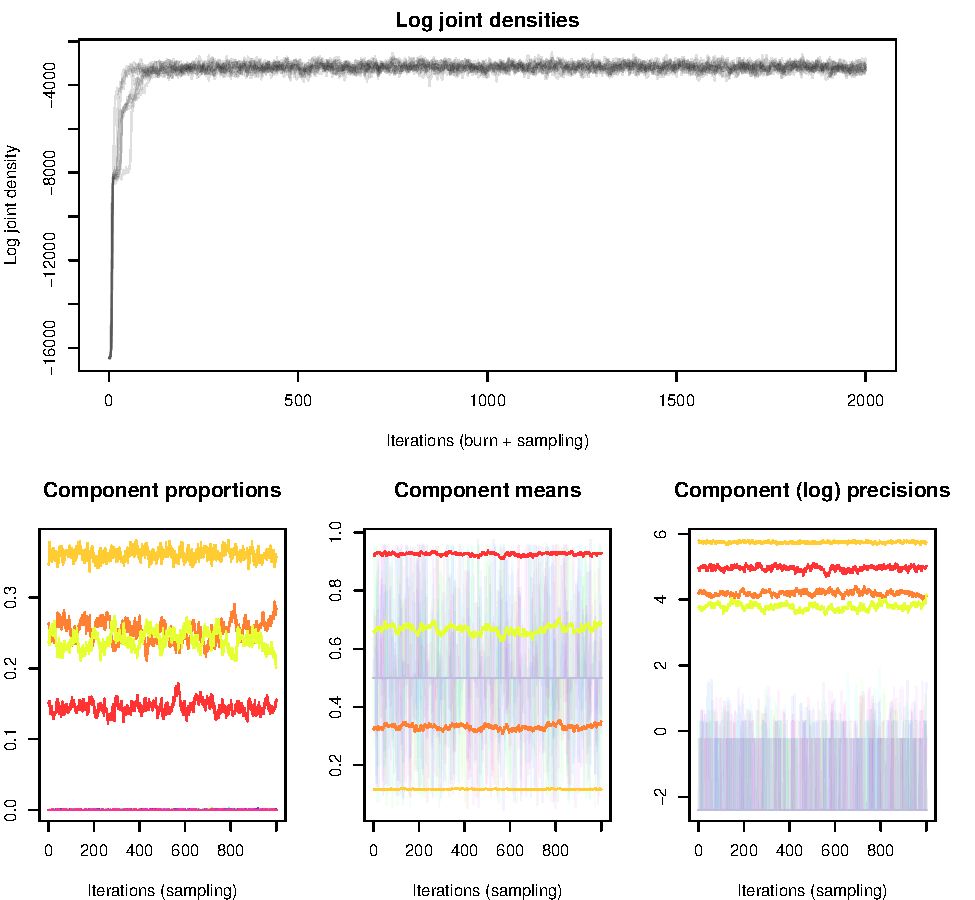
\includegraphics{iotd_logjoint}
\end{center}
\caption{
    \emph{Top}: Evolution of the log joint density $\log{p(\bm{x}_{in},
    \bm{z}_s, \pi_s)}$ over posterior samples $\{(\bm{z}_s, \pi_s)\}$
    (including burn-in), for $8$ chains. \\
    \emph{Bottom Left}: Evolution of cluster proportions $\{\pi_s\}$ over
    sampling iterations for the first chain.
    Only four out of $K = 16$ components are significantly large. \\
    \emph{Bottom Middle}: Evolution of cluster centers $\{m_{k,s}\}$ over sampling
    iterations for the first chain.
    Only the four significantly large clusters have stable centers, with the
    rest (drawn with faded colors) oscillating wildly around the prior mean
    $m_0 = 0$. \\
    \emph{Bottom Right}: Evolution of cluster log precisions
    $\{\log{s_{k,s}^{-2}}\}$ over sampling iterations for the first chain.
}
\label{fig:iotd_joint}
\end{figure}



\begin{figure}[h!]
\begin{center}
    \vspace{1em}
    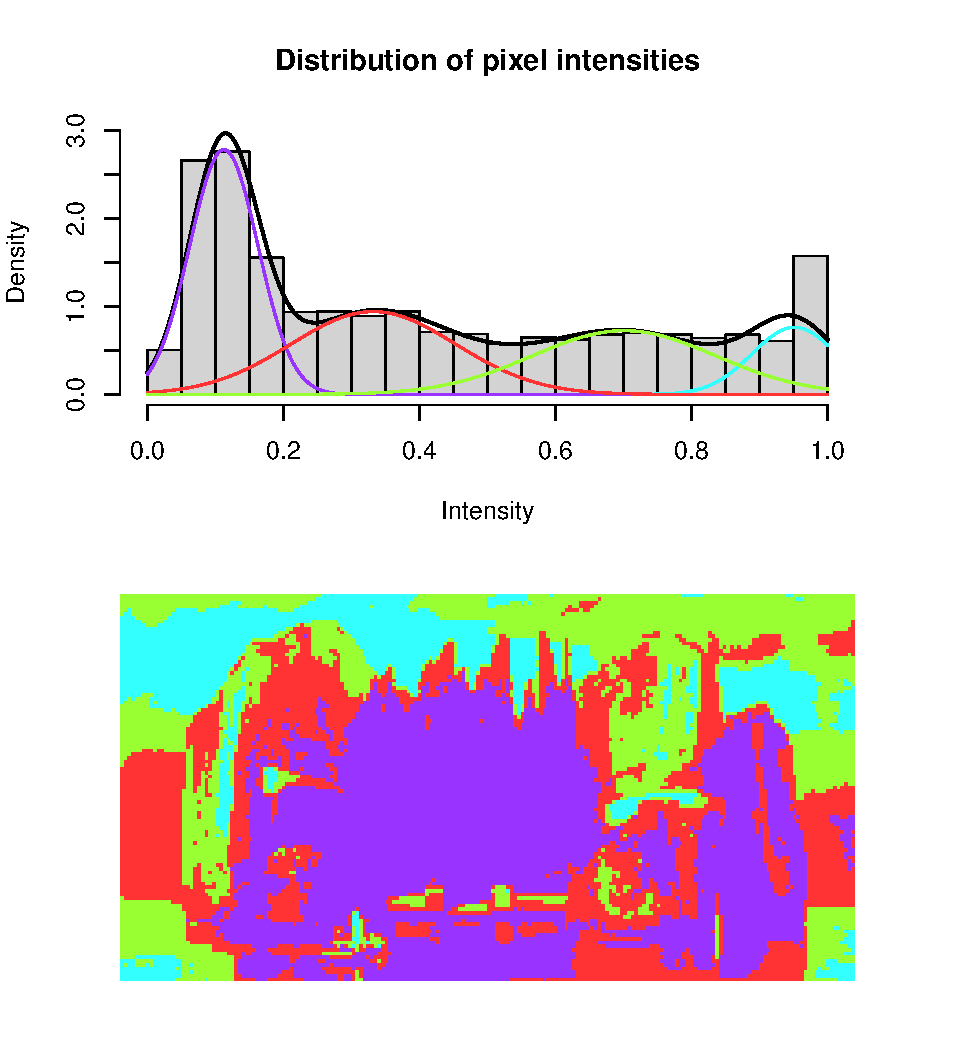
\includegraphics{iotd_data}
\end{center}
\caption{
    \emph{Top}: Histogram of pixel intensities in the image from
    Figure~\ref{fig:iotd} (left).
    The black curve shows the posterior predictive density from fitting a $K =
    4$ Gaussian mixture; the purple, red, green, and blue curves are its
    $t$-distributed components.
    Each of the latter has a degree of freedom so large that it is Gaussian for
    all practical purposes. \\
    \emph{Bottom}: Segmented image --- each pixel is colored according to its
    cluster label.
}
\label{fig:iotd_density}
\end{figure}


\subsection*{Data and setup}

The image in Figure~\ref{fig:iotd} (left) consists of $N = 200\times 105 =
21000$ pixels, each described as an intensity $x_i \in [0, 1]$, with $0$
corresponding to black, $1$ to white.
This is obtained by scaling down a black-and-white of the painting \emph{Isle
of the Dead} to $200\times 105$ pixels and converting it into grayscale (using
ImageMagick).

When fitting our model, we choose prior parameters $m_0 = 0.5$, $a_0 = b_0 =
1$, $\kappa_0 = 0.1$, $\alpha = \bm{1}$.
These have been chosen to be fairly non-informative; the sheer amount of data
makes precise choice of these parameters largely redundant.

We first randomly sample $N_{in} = 10000$ pixels (which is representative of
the full intensity distribution $\bm{x}$) and fit our model with $K = 16$
components, running $8$ chains of collapsed Gibbs sampling; the rest of the
data is held out for validation.
Using this information, we select a suitable number of components $K$ for
fitting our model with the full data and using the sampled cluster labels to
segment our image.
We draw $S = 1000$ posterior samples, after a burn-in period of $1000$
iterations.

The code used to perform these steps can be found in \texttt{gmm.r} and
\texttt{gmm\_img.r}.


\subsection*{Results and diagnostics}

Fitting our model with $K = 16$ on $N_{in} = 10000$ data points, the log joint
densities from all 8 chains quickly reach the same maximum value, which gives
confidence that our sampler has reached stationarity and informs our choice of
a burn-in period: see Figure~\ref{fig:iotd_joint} for traces of log joint
densities, cluster proportions, means, precisions.
The same figure illustrates that only 4 out of 16 component proportions $\pi_k$
stay significantly above zero.
Similarly, only the cluster means and precisions corresponding to these
components remain stable and small.
This shows that the remaining components have little to no contribution in our
overfitted model.
Note that trace plots of the cluster means show no \emph{label switching}.
The chains achieve an estimated \emph{Expected Log Predictive Density} (ELPD)
score of $0.0769 \pm 0.0001$.

With this, we select $K = 4$ for our final fit and segmentation.
The results have been summarized in Figure~\ref{fig:iotd_density}.
The four cluster mean intensities are estimated as $\hat{\bm{m}} = (0.11, 0.33,
0.70, 0.95)$, with proportions $\hat{\pi} = (0.35, 0.29, 0.24, 0.12)$.
Coloring in each segment in the image using its cluster mean $\hat{m}_k$ gives
Figure~\ref{fig:iotd} (right), a fair reconstruction of the original image on
the left using only 4 shades of grey.



\subsection*{Discussion}

Our model reveals that the intensity distribution of Figure~\ref{fig:iotd}
(left) can be decently approximated as a mixture of 4 Gaussians.
This is consistent with the intensity distribution having 4 main modes: see
Figure~\ref{fig:iotd_density}.
The components are not tightly concentrated, and spill over into each other,
reflecting the fact that there aren't many objects in the image which stand out
in large contrast.
The darkest cluster seems to correspond to the trees and their reflection in
the lake, the next to shadows in the cliff and the background, the third to the
lit portion of the cliff and the clouds, and the brightest to the sky,
highlights on the cliff, and the figure on the boat.

The assumption that each component of the intensity distribution is Gaussian is
purely a modeling decision.
There is no \emph{a priori} reason to believe that this is the right choice for
each component; it's just that a Gaussian mixture with sufficiently many
components $K$ is typically flexible enough to capture many distributions, even
though the components themselves may not be entirely interpretable if we allow
$K$ to be very large.
It so happens that we can make do with $K = 4$ here.

The mixture of Gaussians fails to capture the spike in white pixels in the
intensity distribution: the posterior predictive distribution in
Figure~\ref{fig:iotd_density} near $x = 1$ does not peak as sharply as the data
does.
We may model this by adding a mixture component with a point mass at $1$ with
some probability $\pi_0$; this ought to correspond to a Gaussian with a very
large precision.
It is possible that with more careful tuning of hyperparameters and longer
sampling, such a component would be naturally captured with our existing model.

For future work, this model can be extended to a multivariate mixture of
Gaussians, to capture the distribution of pixel RGB values $\bm{x}_i \in [0,
1]^3$ in color images.
An entirely different model taking into account the spatial structure of an
image, modeling each pixel's color as a function of both its component label
and location in the image, is also possible.










\clearpage

\section*{Question 4}



Consider a collection of reviews such as in
\href{https://archive.ics.uci.edu/dataset/331/sentiment+labelled+sentences}{Sentiment Labeled Sentences (Dimitrios Kotzias)},
with each review consisting of a collection of words (text) and a label
indicating its sentiment (positive or negative).
Some basic examples from the dataset are given below.

\begin{table}[ht]
    \centering
    % \caption{
    %     Selected examples from the dataset
    %     \cite{sentiment_labelled_sentences_331}.
    % }
    \vspace{1em}
    \label{tab:review_examples}
    \begin{tabular}{rp{4cm}p{4cm}}
    \toprule
    Source & Positive & Negative \\\midrule
    {Amazon} &
    Very good stuff for the price. &
    Terrible product, and waste of money! \\
    {IMDb} &
    Simply beautiful. &
    Regardless, the film fails on most levels. \\
    {Yelp} &
    It's a great place and I highly recommend it. &
    The service was terrible though. \\\bottomrule
    \end{tabular}
\end{table}

By creating a vocabulary of $V$ words, we could describe each review as a
sequence of words $(w_1, \dots, w_n)$, with a sentiment label $z \in \{0, 1\}$.
If we are willing to ignore the sequential structure of each sentence, we could
view each review as a `bag of words' $\bm{x}$ with $x_v$ denoting the number of
occurrences of the word $v$; normalizing $x_v$ to the relative frequency of $v$
in the review gives a representation $\bm{x} \in \Delta^{V - 1}$ of each review
as a distribution over words.
In this manner, each data entry in this dataset is an element of $\Delta^{V -
1} \times \{0, 1\}$.

A natural task is learning the relationship between each sentence and its
sentiment: can we learn a map $\phi\colon \Delta^{V - 1} \to [0, 1]$ so that we
can model $\mathbb{E}[z \mid \bm{x}] = \phi(\bm{x})$?
We would certainly expect some manner of correlation between the contents of a
sentence and the sentiment it expresses, so this \emph{classification} task
seems possible.
On the other hand, a word distribution $\bm$ may not be enough to generally
infer its sentiment $z$, as the order of words can play a role.

Another task involves learning a lower dimensional latent structure in the
sentences $\bm{x}$, i.e.\ \emph{topic modeling}: can we represent each
review-word distribution $\bm{x}^{V - 1}$ as an $\bm{\ell} \in \Delta^{K - 1}$
mixture of topic-word distributions $\bm{f}_1, \dots, \bm{f}_k \in \Delta^{V -
1}$?
This amounts to `factorizing' our collection $X$ of review-word distributions
as the product $LF^\top$ of latent review-topic distributions $L$ and
topic-word distributions $F$.
Each review $\bm{x}$ gets a local latent variable $\bm{\ell}$ living in a much
lower dimensional space; the topic-word distributions $F$ are global latent
variables which constrain where in $\Delta^{V - 1}$ each sentence $\bm{x}$ can
live.
Models like \emph{Latent Dirichlet Allocation} (LDA) and \emph{Non-negative
Matrix Factorization} (NMF) can answer these questions.

With this dimensionality reduction, we may ask the same question of
classification again: can we learn a map $\varphi\colon \Delta^{K - 1} \to [0,
1]$ such that $\mathbb{E}[z\mid \bm{x}] = \varphi(\bm{\ell}_x)$?
Such a map would show how sentiment depends on \emph{topics} rather than
individual \emph{word} proportions, which is perhaps more interpretable: what
topic $\bm{f}_k$ most affects the inferred sentiment, i.e\ how sensitive is
$\varphi$ to $\ell_k$?
Learning such a map would fall under tasks such as \emph{supervised topic
modeling}; supervised variants of the topic models mentioned above exist to
answer these questions.

















% \clearpage

% \appendix
% \section{Code listing}
% \label{sec:code}

% \texttt{gmm.r}
% \lstinputlisting[language=R]{gmm.r}

% \texttt{gmm\_test.r}
% \lstinputlisting[language=R]{gmm_test.r}

% \texttt{gmm\_img.r}
% \lstinputlisting[language=R]{gmm_img.r}


\end{document}
